% Created 2015-02-04 mié 17:22
\documentclass[xcolor={usenames,svgnames,dvipsnames}]{beamer}
\usepackage[utf8]{inputenc}
\usepackage[T1]{fontenc}
\usepackage{fixltx2e}
\usepackage{graphicx}
\usepackage{longtable}
\usepackage{float}
\usepackage{wrapfig}
\usepackage{rotating}
\usepackage[normalem]{ulem}
\usepackage{amsmath}
\usepackage{textcomp}
\usepackage{marvosym}
\usepackage{wasysym}
\usepackage{amssymb}
\usepackage{hyperref}
\tolerance=1000
\usepackage{color}
\usepackage{listings}
\usepackage{mathpazo}
\usepackage{gensymb}
\usepackage{amsmath}
\bibliographystyle{plain}
\AtBeginSubsection[]{\begin{frame}[plain]\tableofcontents[currentsubsection,sectionstyle=show/shaded,subsectionstyle=show/shaded/hide]\end{frame}}
\AtBeginSection[]{\begin{frame}[plain]\tableofcontents[currentsection,hideallsubsections]\end{frame}}
\usepackage[emulate=units]{siunitx}
\sisetup{per=fraction, fraction=nice, decimalsymbol=comma}
\newunit{\wattpeak}{Wp}
\newunit{\watthour}{Wh}
\newunit{\amperehour}{Ah}
\hypersetup{colorlinks=true, linkcolor=Blue, urlcolor=Blue}
\setbeamercolor{alerted text}{fg=red!50!black} \setbeamerfont{alerted text}{series=\bfseries}
\usetheme[hideothersubsections]{Goettingen}
\usecolortheme{rose}
\usefonttheme{serif}
\author{Oscar Perpiñán Lamigueiro \\ \url{http://oscarperpinan.github.io}}
\date{}
\title{SFB: Componentes}
\hypersetup{
  pdfkeywords={},
  pdfsubject={},
  pdfcreator={Emacs 24.4.1 (Org mode 8.2.7c)}}
\begin{document}

\maketitle

\section{Introducción}
\label{sec-1}

\begin{frame}[label=sec-1-0-1]{Agua y ESF}
\begin{itemize}
\item Las \alert{curvas de generación fotovoltaica y de consumo de agua están
bien adaptadas}: las épocas de mayor calor y radiación solar son de
mayor consumo de agua.

\item Se puede utilizar el \alert{agua como medio de acumulación de energía},
evitando baterías con el consiguiente ahorro de costes, a la vez que
aumenta la seguridad, eficiencia y fiabilidad.

\item El bombeo de agua directo fotovoltaico es limpio: *no presenta los
riesgos de una contaminación del pozo a causa de posibles derrames de
combustible*. Asimismo, se evitan los problemas logísticos de
suministro y transporte de carburante.
\end{itemize}
\end{frame}


\begin{frame}[label=sec-1-0-2]{Composición}
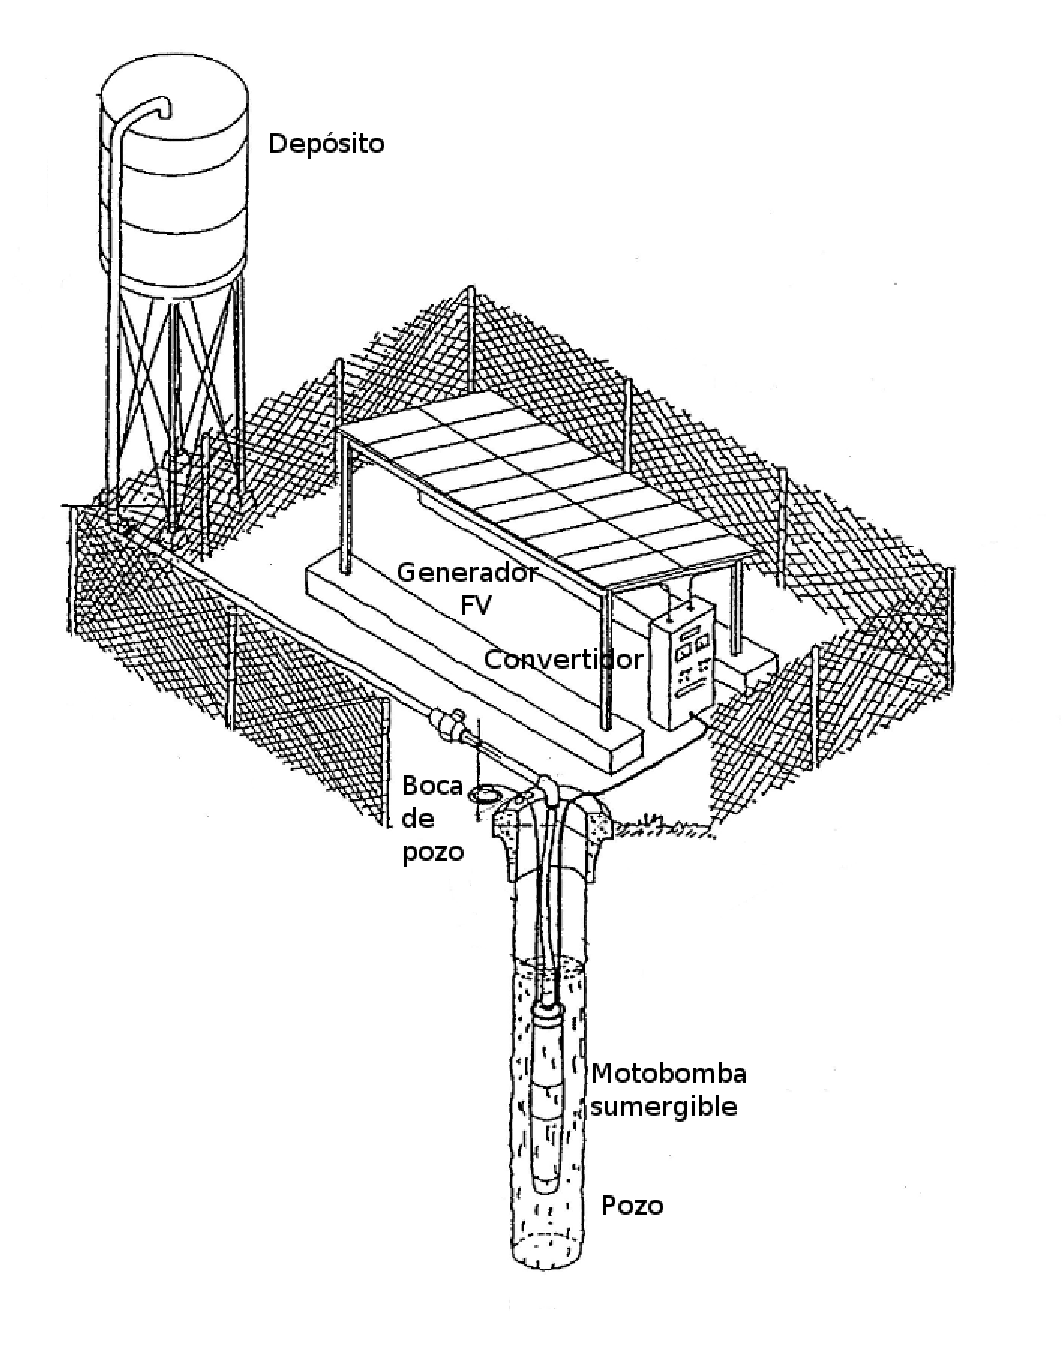
\includegraphics[width=.9\linewidth]{../figs/EsquemaBombeo_oscar.pdf}
\end{frame}

\section{Motobombas}
\label{sec-2}

\begin{frame}[label=sec-2-0-1]{Definición}
\begin{itemize}
\item Un \alert{motor eléctrico} es una máquina eléctrica que \alert{transforma energía
eléctrica en energía mecánica} por medio de interacciones
electromagnéticas.

\item Una \alert{bomba} es una \alert{máquina hidráulica} generadora que* transforma la
energía mecánica* con la que es accionada \alert{en energía hidráulica del
fluido} (agua). Al incrementar la energía del fluido, se aumenta su
presión, su velocidad o su altura, todas ellas relacionadas según el
principio de Bernoulli.
\end{itemize}
\end{frame}

\subsection{Motores eléctricos}
\label{sec-2-1}

\begin{frame}[label=sec-2-1-1]{Electromagnetismo}
\begin{itemize}
\item Un \alert{campo magnético} ejerce una \alert{fuerza} sobre una \alert{carga en
movimiento}.

\item Una \alert{corriente eléctrica crea un campo magnético} en torno al
conductor.

\item Un \alert{conductor por el que circula corriente}, situado \alert{en el seno de
un campo magnético}, altera este campo magnético, y \alert{experimenta una
fuerza} que lo expulsa para \alert{disminuir la alteración}.
\end{itemize}
\end{frame}

\begin{frame}[label=sec-2-1-2]{Electromagnetismo}
\begin{itemize}
\item Entre los puntos extremos de una \alert{espira} estática atravesada por
\alert{campo magnético variable}, aparece una \alert{tensión inducida}.

\item Esta tensión es igual a la \alert{variación} (con signo contrario) \alert{del
flujo magnético} que atraviesa la espira.

\item Si la espira se cierra, \alert{circulará una corriente} que, a su vez,
creará un campo magnético que contrarrestará la variación de flujo.

\item Al circular corriente, la espira experimentará un \alert{par de giro}.

\begin{itemize}
\item \alert{Resultado aprovechable} del motor en forma de potencia mecánica.

\item Restablecer el equilibrio existente antes, intentando \alert{alinear los
ejes magnéticos de inductor e inducido}.
\end{itemize}
\end{itemize}
\end{frame}



\begin{frame}[label=sec-2-1-3]{Motores}
Estator, rotor, inducido e inductor

\begin{itemize}
\item El elemento que permanece fijo es el estator y el que realiza el giro
es el rotor.

\item Según el tipo de motor, el rotor puede ser el inducido y el estator
el inductor o viceversa.
\end{itemize}

Frecuencia eléctrica y velocidad

$$\begin{aligned}
f_{2} & = & f_{1}-n\cdot p\end{aligned}$$

\begin{itemize}
\item $f_{2}$ es la frecuencia en el inducido; $f_{1}$ es la frecuencia en
el inductor; $n$ es la velocidad angular; $p$ es el número de polos.

\item Al utilizar colector de delgas (escobillas) en el inducido, la
frecuencia en el circuito exterior ($f_{L}$) es diferente a $f_{2}$.
\end{itemize}
\end{frame}

\begin{frame}[label=sec-2-1-4]{Tipos de motores en ESF}
Motor DC

\begin{itemize}
\item $f_{1}=0$; $f_{L}=0$;

\item \alert{Estator-Inductor} alimentado por \alert{corriente DC} (o imanes
permanentes).

\item El \alert{colector de delgas} transforma la frecuencia de alimentación (DC)
en alterna.

\item \alert{Rotor-Inducido gira sincronizado} con la frecuencia \guillemotleft{}transformada\guillemotright{}.
\end{itemize}
\end{frame}

\begin{frame}[label=sec-2-1-5]{Tipos de motores en ESF}
Motor DC

\begin{itemize}
\item Los \alert{motores DC con escobillas están sometidos a desgaste}. Necesitan
mantenimiento y por tanto deben evitarse con bombas sumergidas.

\item Existen \alert{motores DC sin escobillas}, donde la conmutación se realiza
mediante un \alert{circuito electrónico}.

\item No necesitan inversor, tienen buen rendimiento, pero están indicados
para \alert{potencias bajas}.
\end{itemize}
\end{frame}

\begin{frame}[label=sec-2-1-6]{Tipos de motores en ESF}
Motor asíncrono o de inducción

\begin{itemize}
\item $f_{1}\neq0$;

\item \alert{Estator-inductor} alimentado por una \alert{corriente trifásica alterna}.
Produce un campo giratorio.

\item \alert{Rotor-inducido} constituido por \alert{espiras cortocircuitadas} (jaula de
ardilla).

\item Se produce un par que busca alinear el eje de las espiras con el
campo inducido. El rotor se mueve siguiendo al campo giratorio.

\item La v*elocidad de giro es inferior a la frecuencia de alimentación*
(asíncrono).
\end{itemize}
\end{frame}

\begin{frame}[label=sec-2-1-7]{Tipos de motores en ESF}
Motor asíncrono o de inducción

\begin{itemize}
\item $f_{2}=f_{1}-n\cdot p$

\item $T\propto\left(\frac{V}{f}\right)^{2}$, $\phi\propto\frac{V}{f}$

\item Son los más comunes, y más baratos que los DC.

\item Tienen \alert{pares de arranque muy bajos}, adecuados para bombas que
requieren bajo par de arranque, como las \alert{centrífugas}.
\end{itemize}
\end{frame}

\subsection{Bombas}
\label{sec-2-2}

\begin{frame}[label=sec-2-2-1]{Ecuación de Bernouilli}
Conservación de energía

$$\frac{\Delta p}{\rho}+\frac{\Delta v^2}{2}+g\cdot\Delta h=cte.$$
\end{frame}

\begin{frame}[label=sec-2-2-2]{Bombas de desplazamiento positivo}
Principio: cambio de presión

El aumento de presión se realiza por el empuje de las paredes de las
cámaras que varían su volumen.

\begin{itemize}
\item \alert{Bombas de émbolo alternativo}, en las que existe uno o varios
compartimentos fijos, pero de volumen variable, por la acción de un
émbolo o de una membrana (bombas de pistones)

\item \alert{Bombas volumétricas}, en las que una masa fluida es confinada en uno
o varios compartimentos que se desplazan desde la zona de entrada (de
baja presión) hasta la zona de salida (de alta presión) de la
máquina. (p.ej. bomba de tornillo).
\end{itemize}
\end{frame}

\begin{frame}[label=sec-2-2-3]{Bombas helicoidales y de membrana}
\begin{itemize}
\item Formadas por un \alert{contorno móvil} que obliga al fluido a avanzar por
la máquina por \alert{cambios de volumen}.

\item Son apropiadas para \alert{altos incrementos de presión y bajos caudales}.
Necesitan un \alert{elevado par de arranque} (por tanto no pueden ser
acopladas directamente al generador).

\item Las bombas de diafragma, más económicas, requieren el \alert{reemplazo de
los diafragmas} cada dos o tres años, dependiendo del fabricante.
\end{itemize}
\end{frame}

\begin{frame}[label=sec-2-2-4]{Bombas de membrana}
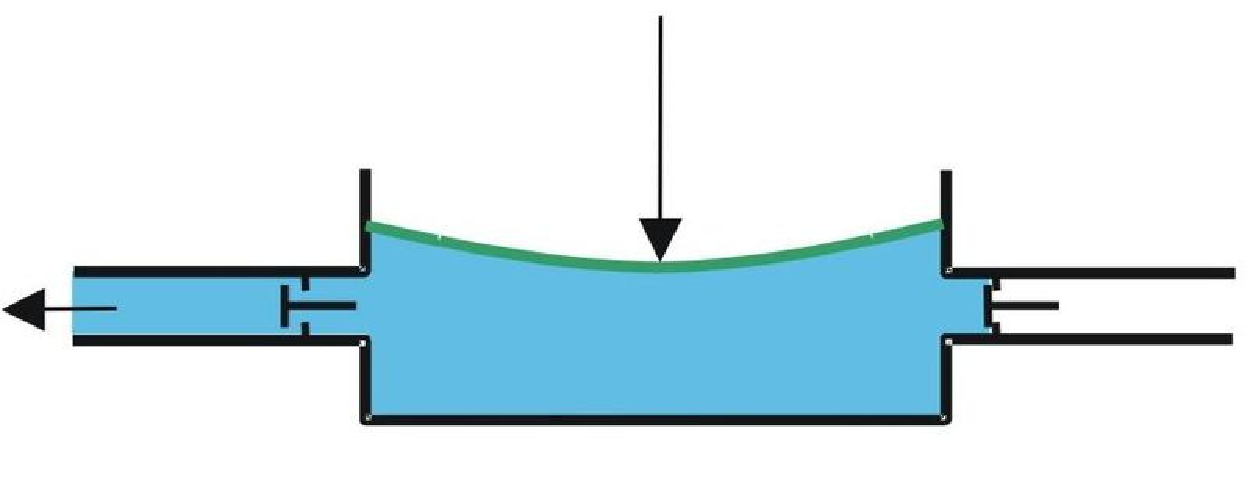
\includegraphics[width=.9\linewidth]{../figs/800px-Bomba_diafragma_impulsando.pdf}

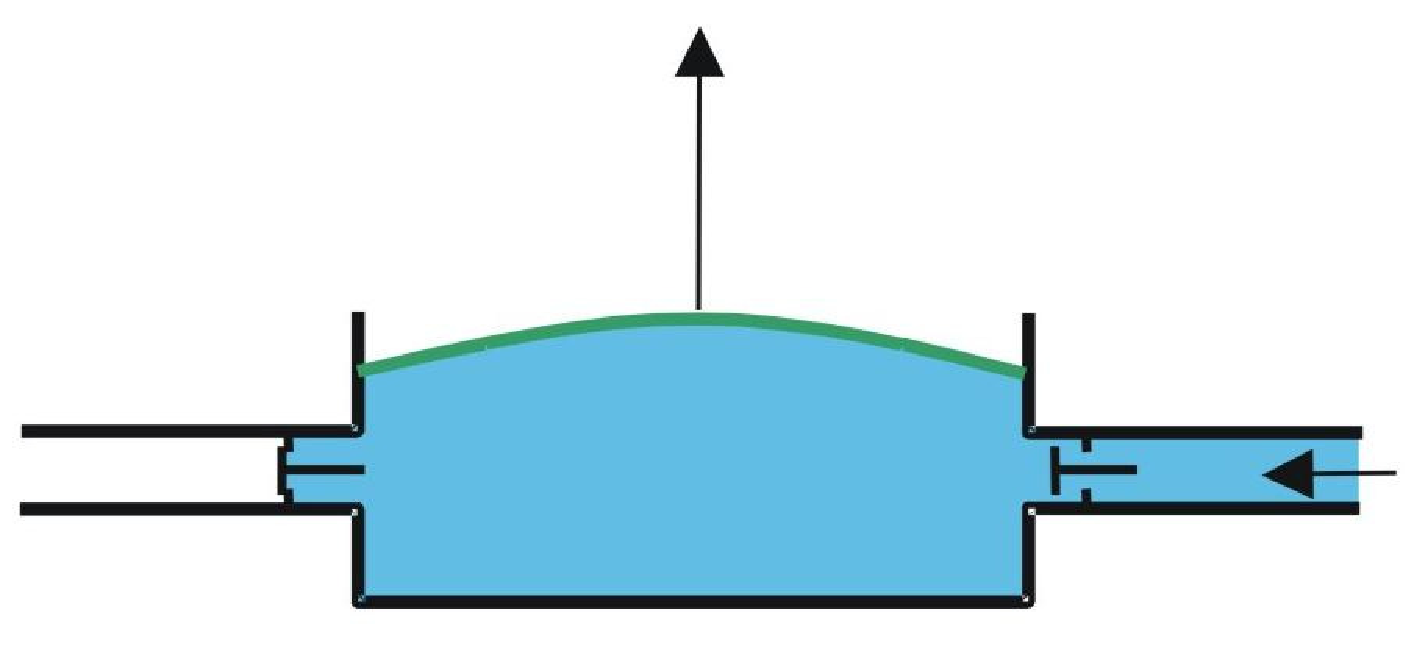
\includegraphics[width=.9\linewidth]{../figs/Bomba_diafragma_aspirando.pdf}
\end{frame}

\begin{frame}[label=sec-2-2-5]{Bombas helicoidales}
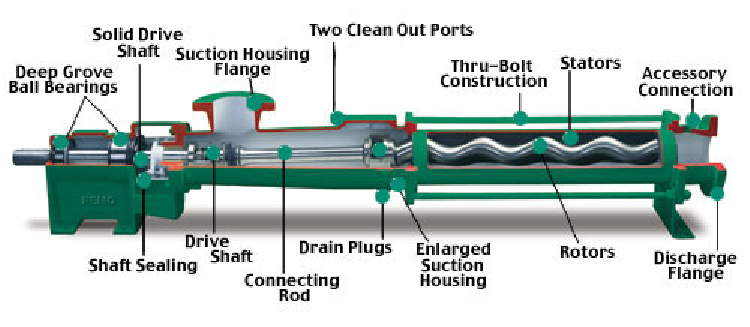
\includegraphics[width=.9\linewidth]{../figs/bombatornillo.pdf}
\end{frame}

\begin{frame}[label=sec-2-2-6]{Bombas rotodinámicas}
Principio: añadir cantidad de movimiento

En este tipo de bombas hay uno o varios rodetes con álabes que giran
generando un campo de presiones en el fluido.

\begin{itemize}
\item \alert{Radiales o centrífugas}, el fluido entra por el centro del rodete,
que dispone de unos álabes para conducir el fluido, y por efecto de
la fuerza centrífuga es impulsado hacia el exterior, donde es
recogido por la carcasa o cuerpo de la bomba, que por el contorno su
forma lo conduce hacia las tubuladuras de salida o hacia el siguiente
rodete (siguiente etapa)
\end{itemize}
\end{frame}

\begin{frame}[label=sec-2-2-7]{Bombas centrífugas}
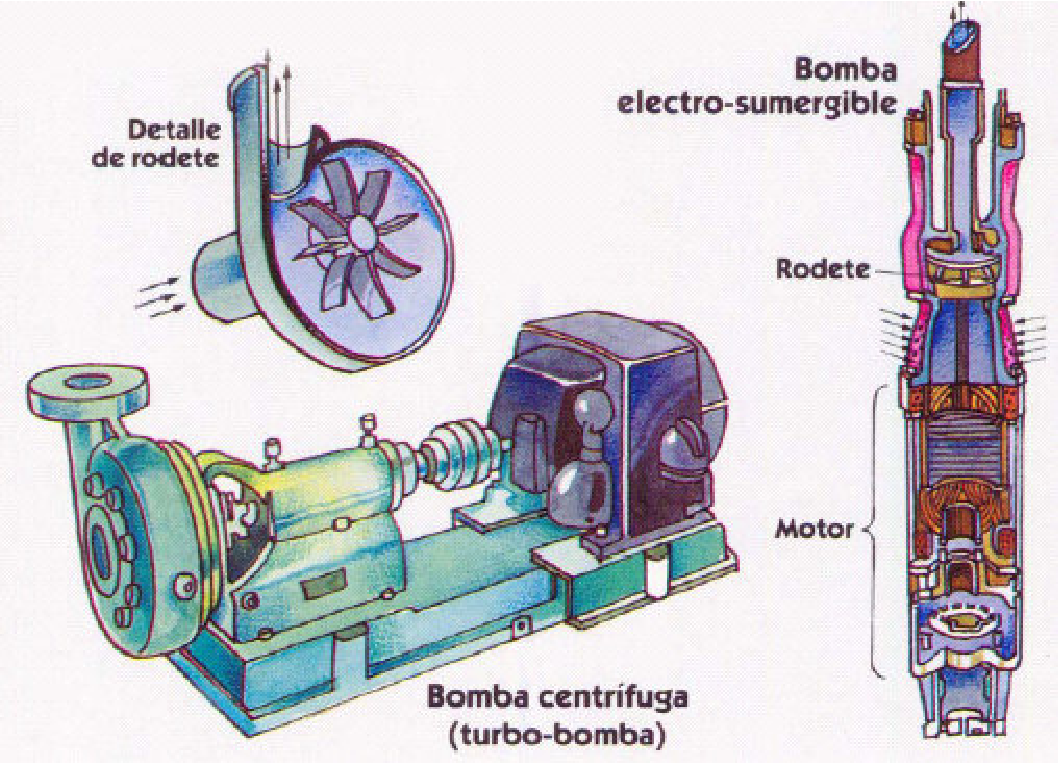
\includegraphics[width=.9\linewidth]{../figs/BombaCentrifuga.pdf}
\end{frame}

\begin{frame}[label=sec-2-2-8]{Bombas centrífugas}
\begin{itemize}
\item Están diseñadas para vencer una \alert{presión más o menos constante},
proporcionando \alert{elevados caudales para bajas alturas manométricas}.

\item Se puede aumentar la altura que son capaces de vencer añadiendo
etapas en serie en la misma bomba.

\item Son \alert{bombas simples y robustas, de bajo coste}.

\item Funcionan bien con pequeños pares de arranque.
\end{itemize}
\end{frame}

\begin{frame}[label=sec-2-2-9]{Leyes de la semejanza}
\begin{block}{Bombas centrífugas}
Rendimiento constante

$$\begin{aligned}
Q & \propto & n\\
H & \propto & n^{2}\\
P_{mec} & \propto & n^{3}\\
T & \propto & n^{2}\end{aligned}$$
\end{block}
\end{frame}

\begin{frame}[label=sec-2-2-10]{Según la disposición}
\begin{itemize}
\item \alert{Bombas sumergibles}

\begin{itemize}
\item Pozos profundos de pequeño diámetro

\item Normalmente ensambladas con el motor.
\end{itemize}

\item \alert{Bombas flotantes}

\begin{itemize}
\item Instalación en ríos, lagos o pozos de gran diámetro en flotación.

\item Mucho caudal pero poca altura manométrica
\end{itemize}

\item \alert{Bombas de superficie}

\begin{itemize}
\item Instaladas a nivel de suelo (fácil mantenimiento)

\item Tienen un límite en el nivel de succión (8 metros).

\item Si utilizan agua como lubricante, no deben operar en seco para
evitar el sobrecalentamiento.
\end{itemize}
\end{itemize}
\end{frame}

\subsection{Acoplamiento motor-bomba}
\label{sec-2-3}

\begin{frame}[label=sec-2-3-1]{Motobombas típicas}
\begin{itemize}
\item Motobomba sumergible, motor AC y bomba centrífuga multietapa.

\item Bomba sumergible, con motor en superficie.

\item Motobomba flotante, con bomba centrífuga.

\item Motor DC y bomba centrífuga flotante.
\end{itemize}
\end{frame}

\begin{frame}[label=sec-2-3-2]{Configuraciones típicas}
\begin{itemize}
\item \alert{Sistemas de baja potencia (50 a 400 Wp)}

\begin{itemize}
\item Motor DC accionando una bomba de membrana

\item Convertidor DC/DC entre generador y motobomba
\end{itemize}

\item \alert{Sistemas de media potencia (400-1500 Wp)}

\begin{itemize}
\item Bomba sumergible centrífuga multietapa con motor asíncrono;
variador de frecuencia.

\item Motor DC sin escobillas accionando una bomba helicoidal;
controlador externo DC.
\end{itemize}

\item \alert{Potencia superior a 1 kWp}

\begin{itemize}
\item Bomba sumergible centrífuga multietapa con motor asíncrono;
variador de frecuencia.

\item Motobomba sumergible
\end{itemize}
\end{itemize}
\end{frame}



\begin{frame}[label=sec-2-3-3]{}
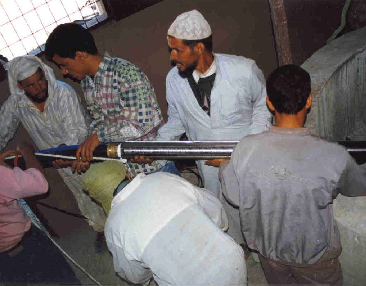
\includegraphics[width=.9\linewidth]{../figs/Marruecos4.pdf}
\end{frame}

\section{Acoplamiento generador-motobomba}
\label{sec-3}

\begin{frame}[label=sec-3-0-1]{Motivo}
\begin{itemize}
\item La \alert{potencia y tensión suministrada por un generador FV varían} con
la radiación y la temperatura.

\item Las condiciones de funcionamiento \alert{no se adaptan siempre a todos los
requerimientos de la motobomba}.

\item Es necesario adaptar las condiciones de funcionamiento de la
motobomba al punto de trabajo del generador FV.

\begin{itemize}
\item \alert{Motor AC: variador de frecuencia}

\item \alert{Motor DC: convertidor DC-DC.}
\end{itemize}
\end{itemize}
\end{frame}

\begin{frame}[label=sec-3-0-2]{Convertidor DC-DC}
\begin{itemize}
\item Dispositivo que \alert{transforma corriente continua de una tensión a
otra}. Suelen ser reguladores de conmutación, dando a su salida una
tensión regulada.

\item Se utiliza para alimentar \alert{motores DC con generador FV}.

\item Normalmente no incorporan buscador de MPP.
\end{itemize}
\end{frame}

\begin{frame}[label=sec-3-0-3]{Variador de frecuencia}
\begin{itemize}
\item El variador de frecuencia* transforma una señal alterna de una
frecuencia en otra señal alterna de otra frecuencia*.

\item Está compuesto por un rectificador y un inversor en serie. El
rectificador convierte la señal de entrada en continua, y el inversor
transforma de nuevo en alterna a la frecuencia deseada.

\item En sistemas FV puede evitarse la pérdida debida al rectificador
entrando directamente al inversor, o bien puede asumirse esta pérdida
y entrar al rectificador, lo que sirve como protección contra
inversión de polaridad.

\item El rendimiento de un variador a una tensión cercana a la nominal
oscila entre el 94 y el 95\%.
\end{itemize}
\end{frame}

\begin{frame}[label=sec-3-0-4]{Variador de frecuencia}
\begin{itemize}
\item Realiza \alert{continuas variaciones en la tensión de generador para
alcanzar un valor de referencia}.

\item Para conseguir igualar la tensión de generador y referencia, varía la
frecuencia.

\item No suele realizarse seguimiento del punto de máxima potencia (MPP),
ni por temperatura ni por radiación.
\end{itemize}
\end{frame}

\begin{frame}[label=sec-3-0-5]{Variador de frecuencia}
$$T_{max}=k_{T}\left(\frac{V_{1}}{f_{1}}\right)^{2}$$

$$\phi\simeq k_{\phi}\frac{V_{1}}{f_{1}}$$

\begin{itemize}
\item Par constante: $\frac{V_{1}}{f_{1}}=\mathrm{cte.}$

\item Par cuadrático: $V_{1}=k_{V}\cdot f_{1}^{2}$
\end{itemize}
\end{frame}

\begin{frame}[label=sec-3-0-6]{Protecciones}
Pozo vacío

\begin{itemize}
\item \alert{Control de frecuencia de salida del variador}.

\item Cuando el motor trabaja en vacío, la corriente consumida baja. Por
tanto, el variador debe subir la frecuencia para alcanzar la tensión
de referencia.

\item Si se supera la frecuencia de 55 Hz se para el sistema y se marca un
intervalo de espera para permitir que el pozo vuelva a llenarse.
\end{itemize}
\end{frame}

\begin{frame}[label=sec-3-0-7]{Protecciones}
Deposito lleno

\begin{itemize}
\item \alert{Presostáto en la tubería combinado con una boya en el depósito}.

\item Cuando en el depósito se alcanza un nivel determinado, la boya
acciona el cierre de la entrada al depósito.

\item Sin embargo, la bomba sigue elevando agua. De esta forma, la presión
dentro de la tubería aumenta hasta accionar el Presostáto.

\item Se pone en marcha un temporizador para permitir que baje el nivel del
depósito.
\end{itemize}
\end{frame}



\begin{frame}[label=sec-3-0-8]{}
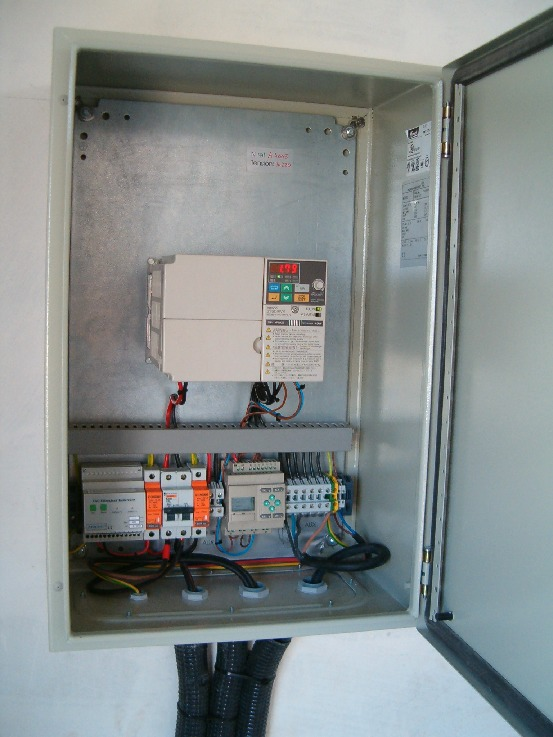
\includegraphics[width=.9\linewidth]{../figs/VariadorFrecuencia.jpg}
\end{frame}

\section{Circuito Hidráulico}
\label{sec-4}

\begin{frame}[label=sec-4-0-1]{Circuito hidráulico}
Es el conjunto de accesorios hidráulicos que completan la instalación
desde la salida del pozo/sondeo hasta el punto de suministro, pasando
por el almacenaje en depósito elevado en caso necesario (reserva para
días de baja o escasa radiación, ya que generalmente se bombea más agua
de la necesaria)

\begin{itemize}
\item Tubería de impulsión

\item Boca de pozo

\item Tubería de distribución y valvulería

\item Depósito
\end{itemize}
\end{frame}

\begin{frame}[label=sec-4-0-2]{}
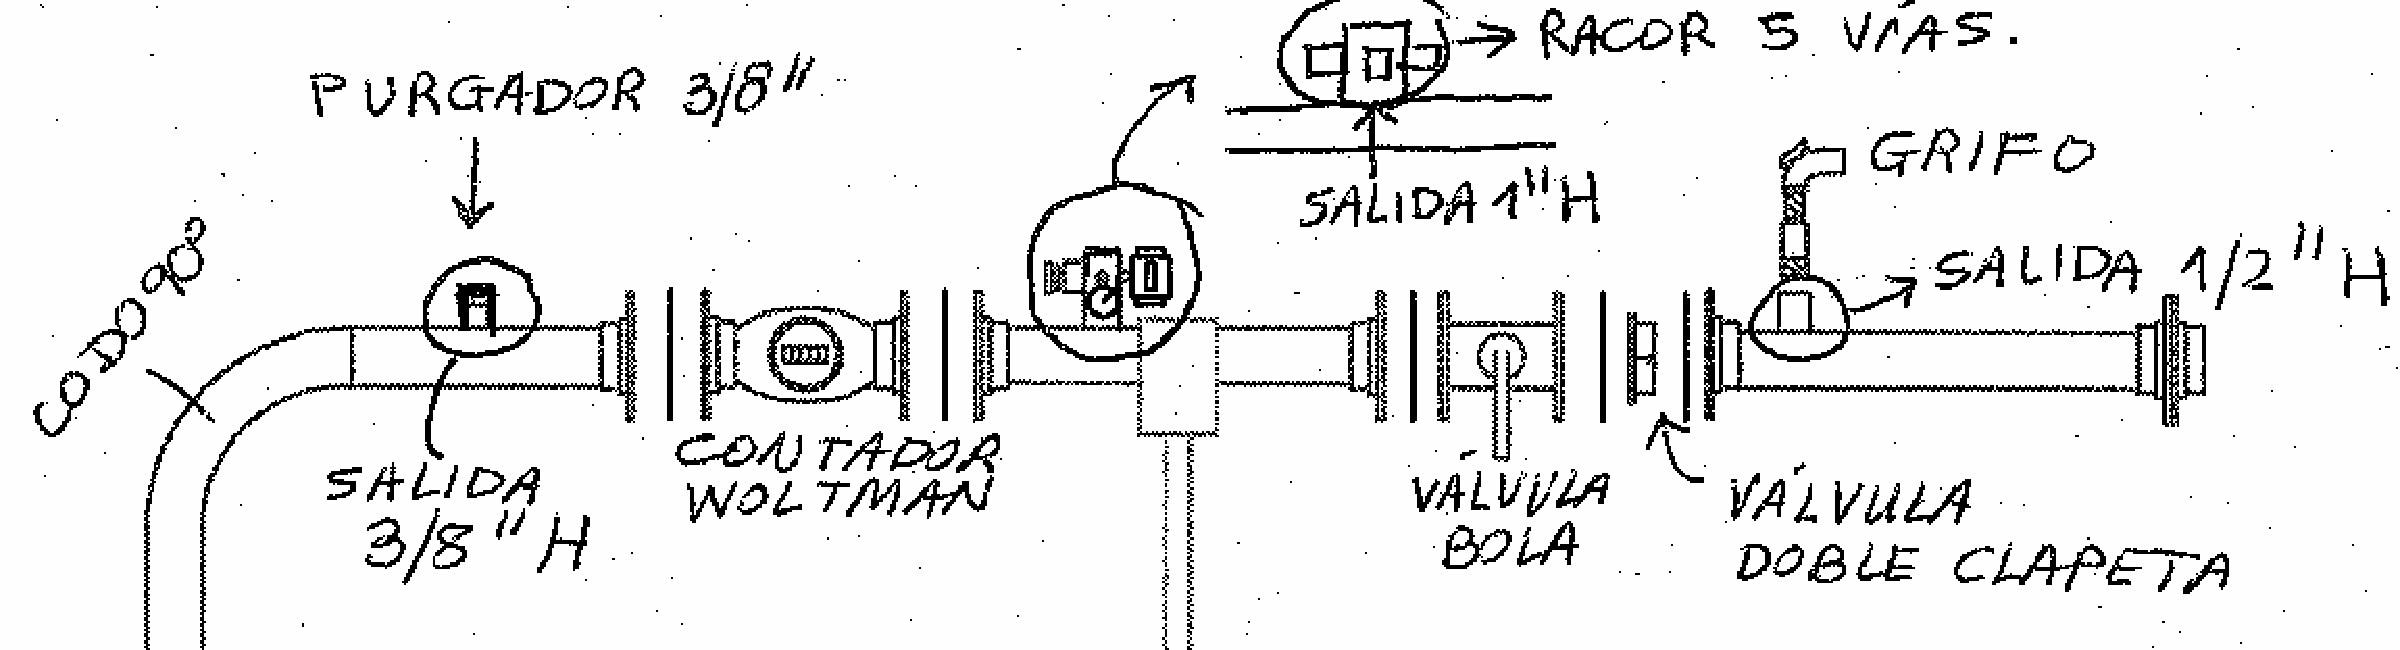
\includegraphics[width=.9\linewidth]{../figs/CircuitoHidraulico.pdf}
\end{frame}

\begin{frame}[label=sec-4-0-3]{Tubería de Impulsión}
\begin{itemize}
\item Es la tubería instalada a la salida de la bomba.

\item Podrá ser de polietileno de alta densidad calidad alimentaria, de
coste menor pero con ciertos problemas a la hora de la instalación
por su tendencia a enrollarse.

\item Como alternativa están las tuberías autoportantes flexibles que
evitan los problemas anteriores, aunque su coste es mayor, además de
requerir terminales específicos fabricados en acero inoxidable que
encarecen la instalación.
\end{itemize}
\end{frame}

\begin{frame}[label=sec-4-0-4]{Depósito elevado}
\begin{itemize}
\item Para depósitos pequeños, de 20 a 1.000 l, para agua potable, debe
elegirse un depósito plástico de color negro, ya que los colores que
transparentan la luz favorecen la aparición de algas y otros
contaminantes.

\item El plástico puede ser polietileno de alta densidad para uso
alimentario.
\end{itemize}
\end{frame}



\begin{frame}[label=sec-4-0-5]{}
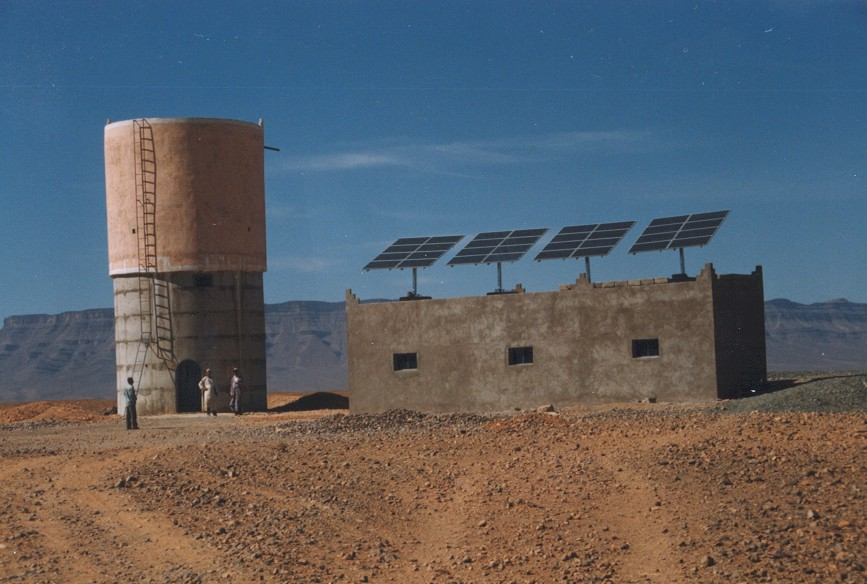
\includegraphics[width=.9\linewidth]{../figs/Bombeo.jpg}
\end{frame}
% Emacs 24.4.1 (Org mode 8.2.7c)
\end{document}